% Figure 1, narrow screens. From Year 1 to an offer. Labels: LABELS.md, Figure 1.
\def\eeprepfigure{1}
\providecommand{\eepstyledir}{../style}% repo: ../style
\input{\eepstyledir/circuitikz-preamble.tex}
% Colours, fonts, and text styles for the Get hired figures.
% Input after style/circuitikz-preamble.tex (in the repo: ../../style/circuitikz-preamble.tex).
% Define \eepdark before this file for the dark build. Same names as the resume figures,
% plus the rest of the navy palette. Crimson (eepaccent) marks one thing per figure.
\setmainfont{Newsreader}[
  BoldFont={Newsreader Bold},
  ItalicFont={Newsreader Italic},
  BoldItalicFont={Newsreader Bold Italic},
]
\usetikzlibrary{arrows.meta,calc,decorations.pathreplacing}
\ifdefined\eepdark
  \definecolor{eepink}{HTML}{ECEEF2}
  \definecolor{eeptext}{HTML}{D0D4DB}
  \definecolor{eepinktwo}{HTML}{A6AFBF}
  \definecolor{eepmute}{HTML}{8F95A0}
  \definecolor{eepsilver}{HTML}{76808F}
  \definecolor{eeprule}{HTML}{3B4352}
  \definecolor{eepwash}{HTML}{17243A}
  \definecolor{eepsunken}{HTML}{101828}
  \definecolor{eepfill}{HTML}{131C2E}
  \definecolor{eeppaper}{HTML}{0D1524}
  \definecolor{eepaccent}{HTML}{E06A5F}
  \definecolor{eepaccentsoft}{HTML}{2A1A24}
\else
  \definecolor{eepink}{HTML}{16233A}
  \definecolor{eeptext}{HTML}{232A39}
  \definecolor{eepinktwo}{HTML}{424D63}
  \definecolor{eepmute}{HTML}{5E636C}
  \definecolor{eepsilver}{HTML}{838C9A}
  \definecolor{eeprule}{HTML}{C4C8CF}
  \definecolor{eepwash}{HTML}{E7ECF3}
  \definecolor{eepsunken}{HTML}{F3F4F6}
  \definecolor{eepfill}{HTML}{FFFFFF}
  \definecolor{eeppaper}{HTML}{FBFBFC}
  \definecolor{eepaccent}{HTML}{A3201D}
  \definecolor{eepaccentsoft}{HTML}{F8ECEA}
\fi
% Draw in y-down points so coordinates read like a mockup: [x=1pt, y=-1pt].
\tikzset{
  eeptitle/.style={anchor=base west, inner sep=0pt, text=eepink, font=\rmfamily\bfseries\fontsize{26}{31}\selectfont},
  eephead/.style={inner sep=0pt, text=eepink, font=\sffamily\bfseries\fontsize{14.5}{18}\selectfont},
  eepbody/.style={inner sep=0pt, text=eepinktwo, font=\sffamily\fontsize{13}{17}\selectfont},
  eepnote/.style={inner sep=0pt, text=eepmute, font=\sffamily\fontsize{12.5}{16}\selectfont},
  eepsrc/.style={anchor=north west, inner sep=0pt, align=left, text=eepmute, font=\sffamily\fontsize{11}{14.5}\selectfont},
  eepbox/.style={draw=eepink, fill=eepfill, rounded corners=4pt},
  eepfocus/.style={draw=eepaccent, fill=eepfill, rounded corners=4pt, line width=1.8pt},
  eeparrow/.style={-{Stealth[length=8pt,width=6pt]}},
  eepdash/.style={dash pattern=on 4pt off 4pt},
  eeplead/.style={draw=eepsilver, line width=0.9pt},
}
% A dot on a trace, like a schematic junction.
\newcommand{\eepdot}[2][eepink]{\fill[#1] #2 circle (3.6pt);}
% Short labels never hyphenate.
\hyphenpenalty=10000 \exhyphenpenalty=10000
% One space after a full stop, as on the site.
\frenchspacing

% #1 name, #2 previous node, #3 heading, #4 lines, #5 heading colour
\newcommand{\tlstop}[5]{%
  \node[anchor=north west, inner sep=0pt, text width=320pt, align=left] (#1) at ($(#2.south west)+(0,20)$)
    {{\sffamily\bfseries\fontsize{14}{17}\selectfont\color{#5}#3\par}\vspace{5pt}%
     {\sffamily\fontsize{13}{17}\selectfont\color{eepinktwo}#4\par}};
  \fill[#5] ($(#1.north west)+(-26,7)$) circle (3.8pt);}
\newcommand{\gap}{\par\vspace{4pt}}
\begin{document}
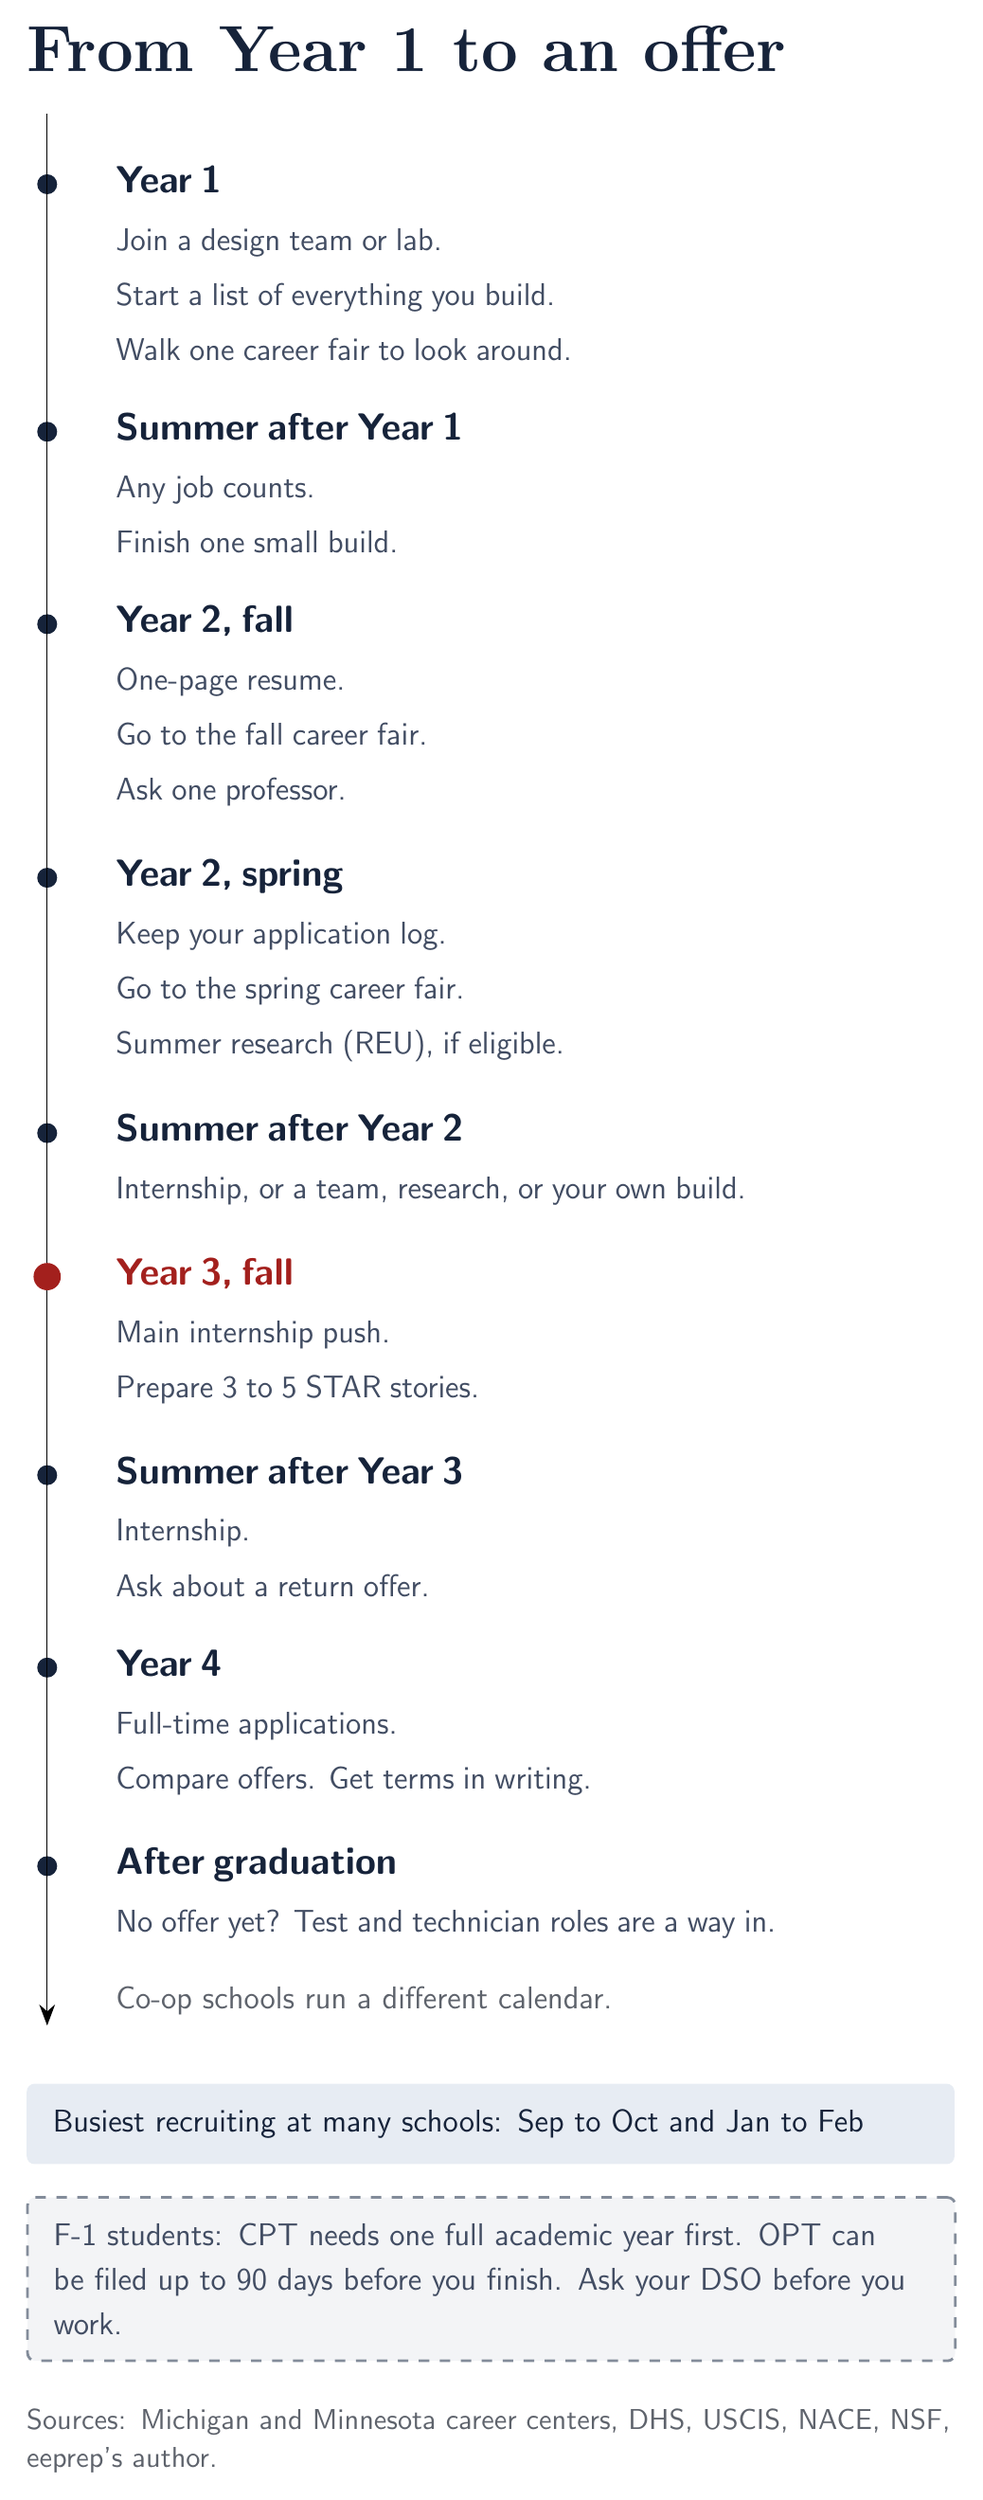
\begin{tikzpicture}[x=1pt,y=-1pt]
  \node[eeptitle] at (0,30) {From Year 1 to an offer};
  \coordinate (s0) at (34,46);
  \tlstop{s1}{s0}{Year 1}{Join a design team or lab.\gap Start a list of everything you build.\gap Walk one career fair to look around.}{eepink}
  \tlstop{s2}{s1}{Summer after Year 1}{Any job counts.\gap Finish one small build.}{eepink}
  \tlstop{s3}{s2}{Year 2, fall}{One-page resume.\gap Go to the fall career fair.\gap Ask one professor.}{eepink}
  \tlstop{s4}{s3}{Year 2, spring}{Keep your application log.\gap Go to the spring career fair.\gap Summer research (REU), if eligible.}{eepink}
  \tlstop{s5}{s4}{Summer after Year 2}{Internship, or a team, research, or your own build.}{eepink}
  \tlstop{s6}{s5}{Year 3, fall}{Main internship push.\gap Prepare 3 to 5 STAR stories.}{eepaccent}
  \tlstop{s7}{s6}{Summer after Year 3}{Internship.\gap Ask about a return offer.}{eepink}
  \tlstop{s8}{s7}{Year 4}{Full-time applications.\gap Compare offers. Get terms in writing.}{eepink}
  \tlstop{s9}{s8}{After graduation}{No offer yet? Test and technician roles are a way in.}{eepink}
  \node[eepnote, anchor=north west, text width=320pt] (coop) at ($(s9.south west)+(0,18)$) {Co-op schools run a different calendar.};
  % The trace runs down the left edge, behind the junction dots.
  \draw[eeparrow] (8,46) -- ($(coop.south west)+(-26,4)$);
  \fill[eepaccent] ($(s6.north west)+(-26,7)$) circle (5.2pt);
  % Two bands, stacked.
  \node[anchor=north west, text width=334pt, fill=eepwash, rounded corners=3pt, eepbody, text=eepink, align=left, inner sep=10pt] (b1) at ($(coop.south west)+(-34,26)$)
    {Busiest recruiting at many schools: Sep to Oct and Jan to Feb};
  \node[anchor=north west, text width=334pt, fill=eepsunken, draw=eepsilver, line width=1pt, eepdash, rounded corners=3pt, eepbody, align=left, inner sep=10pt] (b2) at ($(b1.south west)+(0,12)$)
    {F-1 students: CPT needs one full academic year first. OPT can be filed up to 90 days before you finish. Ask your DSO before you work.};
  \node[eepsrc, text width=354pt] at ($(b2.south west)+(0,18)$) {Sources: Michigan and Minnesota career centers, DHS, USCIS, NACE, NSF, eeprep's author.};
\end{tikzpicture}
\end{document}
